% header
\documentclass[10pt,a4paper]{article}

\usepackage[utf8]{inputenc}
\usepackage{hyperref}
\usepackage{amssymb}
\usepackage{amsmath}
\usepackage{listings}
\usepackage{graphicx}

% the document
\begin{document}

\title{Worksheet $2$\\
\small{Practical Lab Numerical Computing}}
\author{Andrii Lischishin \and Lars Schleithoff \and Hendrik Kleikamp}
\date{\today}
\maketitle

\section*{Task 7}

Uniform random numbers in $(0,1)^2$:
\begin{center}
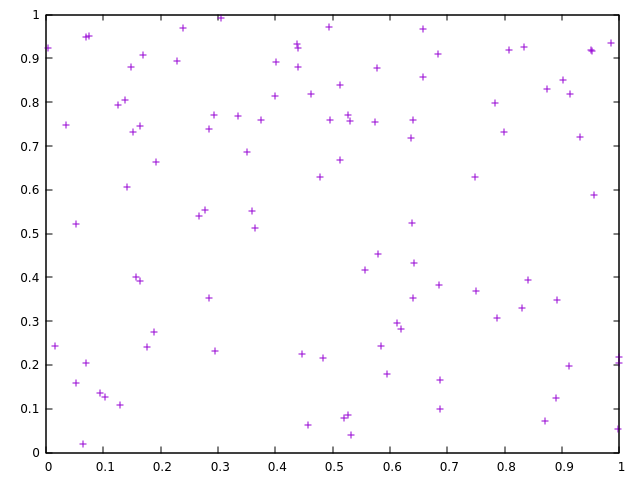
\includegraphics[scale=0.5]{uniform_random_numbers.png}		
\end{center}

Halton sequence:
\begin{center}
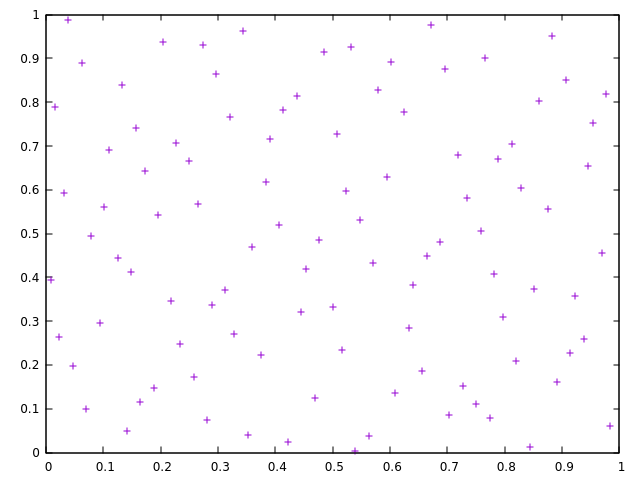
\includegraphics[scale=0.5]{halton_sequence.png}		
\end{center}

One can see that there are some regions in $(0,1)^2$ where no uniform random numbers are set. This is not the case in the point set calculated by the Halton sequence. The Hatlon sequence gives a very uniform distributed set without any holes.

\section*{Task 9}

Qudrature nodes of the two-dimensional product rule for trapezoidal rule:
\begin{center}
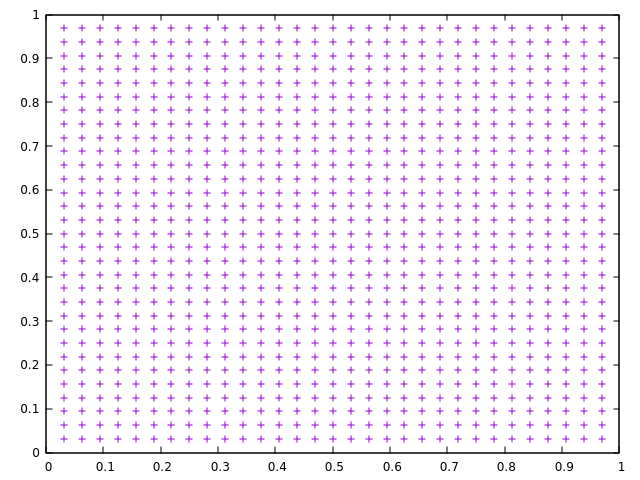
\includegraphics[scale=0.5]{quadrature_nodes_trapezoidal_rule.png}		
\end{center}

Qudrature nodes of the two-dimensional product rule for Gauss-Legendre:
\begin{center}
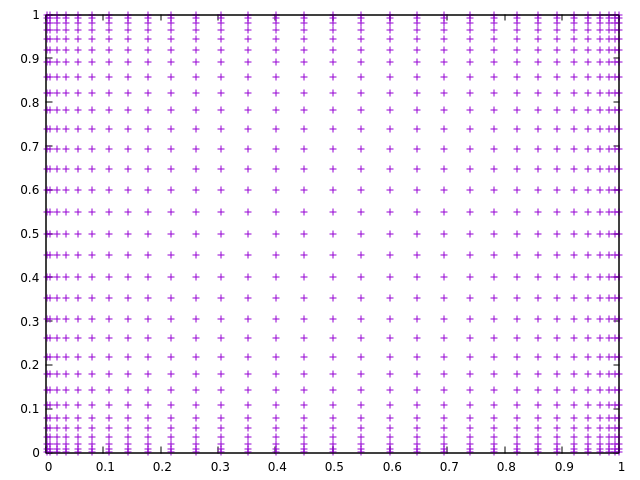
\includegraphics[scale=0.5]{quadrature_nodes_gauss_legendre.png}		
\end{center}

Qudrature nodes of the two-dimensional product rule for Clenshaw Curtis:
\begin{center}
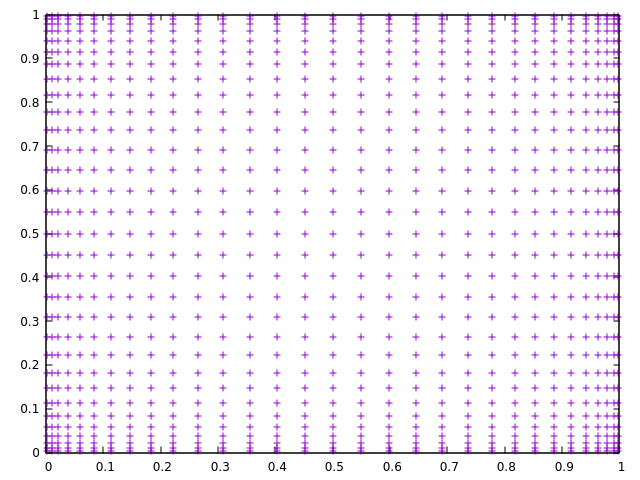
\includegraphics[scale=0.5]{quadrature_nodes_clenshaw_curtis.png}		
\end{center}


\end{document}